\chapter[Trasmissione dei segnali]{Principi di base sulla trasmissione dei segnali: teorema del campionamento e quantizzazione}
\section{Trasmissione dei segnali}
La trasmissione di un segnale è un problema comune presente ogni qual volta è necessario trasportare l'informazione associata ad una grandezza fisica da un punto dello spazio ad un altro. Uno schema generico di un sistema di trasmissione prevede sempre i seguenti elementi base:
\begin{itemize}
	\item un \textsc{trasmettitore}, l'apparato in prossimità della sorgente del segnale, che ha il compito di fornire la potenza necessaria al segnale per attraversare il mezzo trasmissivo e giungere riconoscibile al ricevente;
	\item un \textsc{mezzo trasmissivo}, che rappresenta il mezzo fisico attraverso cui si propaga il segnale trasmesso, le cui caratteristiche possono alterare il messaggio. Esistono due grandi categorie: mezzi ad onde convogliate (non dispersivi), mezzi ad onde irradiate (dispersivi);
	\item un \textsc{ricevitore}, l'apparato in prossimità della destinazione del segnale, che ha il compito di estrarre dal mezzo trasmissivo il segnale utile, ovvero quello che contiene l'informazione che trasporta il messaggio originale.
\end{itemize}
\begin{figure}[!ht]
	\begin{center}\begin{tikzpicture}[node distance=2cm]
		\node [block,minimum width=4cm, minimum height=.5cm] (mt) {$MT$};
		\node [block, left =of mt] (tx) {$T_X$};
		\node [block, right =of mt] (rx) {$R_X$};
		\draw [-latex] (tx) -- (mt);
		\draw [-latex] (mt) -- (rx);
		\end{tikzpicture}
	\end{center}
\end{figure}

I mezzi trasmissivi ad onde irradiate sono lo spazio vuoto e l'atmosfera, attraverso cui si propagano onde elettromagnetiche. Il trasmettitore e il ricevitore sono due antenne che irradiano e ricevono potenza del campo elettromagnetico. Le più semplici sono antenne isotrope in cui la potenza del segnale si distribuisce allo stesso modo in ogni direzione dello spazio, propagando il fronte di una superficie sferica di raggio via via crescente alla velocità delle onde elettromagnetiche nel vuoto $c$.

Ad una distanza $R$ dall'antenna trasmittente la potenza ricevuta è attenuata rispetto alla potenza trasmessa secondo una legge
\begin{equation}
P_R=P_T R^{-\alpha}
\end{equation}
con $\alpha$ indice di attenuazione, compreso tra $\alpha=2$ in spazio aperto e $\alpha=4.5$ in ambienti indoor.

I mezzi trasmissivi ad onde convogliate trasmettono la potenza del segnale di tensione o di corrente attraverso sistemi a cavo, come doppino in rame, cavo coassiale, fibra ottica. Per le loro dimensioni non possono essere studiati come circuiti a parametri concentrati e bisogna tener conto degli effetti dissipativi e di ritardo di un mezzo a costanti distribuite.
La potenza trasmessa risulta attenuata, secondo le leggi fisiche del mezzo, in modo lineare con la distanza in unità logaritmiche
\begin{equation}
P_R=P_T\cdot{10}^{-\alpha_\text{TOT}}
\end{equation}
Esprimendo la potenza in decibel
\[P_{R\text{[dB]}}=10\Log P_R=10\Log P_T-\alpha_\text{TOT}=P_{T\text{[dB]}}-\alpha_S\cdot\ell \]
dove si è indicato con $\alpha_S$ l'attenuazione specifica in decibel per unità di lunghezza. Per conduttori in metallo l'attenuazione è funzione della frequenza $\left(\alpha_S=\alpha_\text{r}\sqrt{\frac{f}{f_r}}\right)$.

Un mezzo trasmissivo ideale si suppone lineare e tempo-invariante almeno nella banda di interesse. Il segnale trasmesso $s_T(t)$ giunge in uscita attenuato e ritardato, a causa della velocità di propagazione finita, come $s_R(t)=k\cdot s_T(t-t_0)$, ovvero con una funzione di trasferimento in frequenza \[H(f)=k\e{-\imath 2\pi f t_0}\]

Un mezzo trasmissivo reale è solo approssimativamente lineare, e può avere caratteristiche che variano lentamente nel tempo, e una funzione di trasferimento che attenui diversamente alle varie frequenze, \[H(f)=H_T(f)\e{-\imath 2\pi f t_0}\]

Tale comportamento richiede un filtro di equalizzazione in ricezione che compensi l'effetto del mezzo trasmissivo \[H_\text{eq}(f)=\frac{k}{H(f)}\]

Un mezzo trasmissivo reale introduce sempre una qualche forma di disturbo del segnale trasmesso. In ricezione dunque oltre il segnale distorto dal mezzo sarà presente un segnale indesiderato sovrapposto, genericamente indicato come \textsc{rumore}.

\section{Trasmissione analogica e numerica}

I sistemi di trasmissione distinguono tra \textsc{trasmissione analogica} e \textsc{trasmissione numerica}.
Nella trasmissione analogica l'informazione trasmessa è il segnale stesso, come questo è disponibile al trasmettitore.
Nella trasmissione numerica il segnale viene codificato in \textsc{simboli} a cui corrispondono forme d'onda analogiche.

La trasmissione numerica consente di non dover modificare il sistema a seconda del segnale originale da trasmettere. Si riesce a controllare con precisione l'entità dei disturbi in rapporto al segnale codificato. Si risparmia potenza a parità di informazione trasmessa o, equivalentemente, si può trasmettere più informazione a parità di potenza in trasmissione.

Lo schema di trasmissione/ricezione è più complesso. Per rendere un segnale analogico un segnale numerico è necessario eseguire  operazioni di filtraggio, \textsc{campionamento} e \textsc{quantizzazione}.  Operazioni che hanno la caratteristica di essere invertibili per poter tornare al segnale originario dal lato del ricevitore.

\begin{figure}[!h]
	\begin{center}\begin{tikzpicture}
		\node [block,node distance=1cm] (f) {filtro};
		\node [left of= f,node distance=2cm](input) {$s(t)$};
		\node [block, right of= f,node distance=3cm] (c) {campionamento};
		\node [block, right of= c,node distance=4cm] (q) {quantizzazione};
		\node [block,right of= q,minimum width=3cm, minimum height=.5cm,node distance=4cm] (mt) {$MT$};
		\draw [-latex] (input) -- (f);
		\draw [-latex] (f) -- (c);
		\draw [-latex] (c) -- (q);
		\draw [-latex] (q) -- (mt);
		\end{tikzpicture}
	\end{center}
\end{figure}

\section{Campionamento}\label{sec:campionamento}
Dato un segnale analogico l'operazione di campionamento estrae i valori del segnale in istanti discreti del tempo. Si ottiene un segnale numerico, una serie di numeri reali che rappresentano i campioni del segnale. Il numero di campioni deve essere sufficiente a poter ricostruire il segnale originale.

\begin{figure}[!ht]
	\centering
	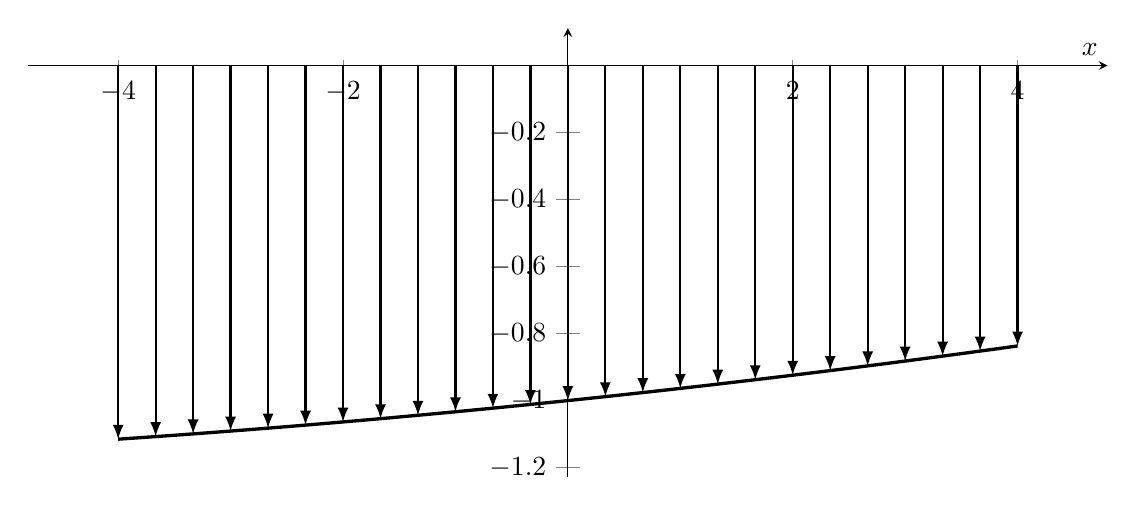
\begin{tikzpicture}
	\begin{axis}[axis lines=middle,no markers,enlargelimits,xscale=2,xtick={},ytick={},xlabel=$x$]
	\addplot+[quiver={u=0,v=-y},latex-,black,thick,samples=25,domain=-4:4] {sin(2*x)-cos(pi*x)};
	\addplot[very thick,samples=200,smooth,domain=-4:4] {sin(2*x)-cos(pi*x)};
	\end{axis}\end{tikzpicture}
	\caption{Campionamento}
\end{figure}

Bisogna dimensionare il passo di campionamento $T$ al fine di avere un numero gestibile di campioni che consenta di ricostruire il segnale senza perdere informazione.

\subsection{Teorema del campionamento}
Per ricostruire fedelmente un segnale con spettro a banda limitata $[-B,B]$ su cui si è operato un campionamento a frequenza $f_S=\frac{1}{T}$ si deve avere $f_S\geq B$.
\begin{proof}[Dim.]
Dato il segnale $s(t)$ con spettro $S(f)$ limitato alle frequenze $f\in[-B,B]$ (in banda base), e data la proprietà dell'impulso di estrarre un campione del segnale, si definisce il segnale campionato $s_C(t)$ come il prodotto tra il segnale $s(t)$ e un treno di impulsi di ampiezza unitaria ad intervalli di tempo regolari di periodo $T$
\begin{equation}
s_C(t)=s(t)\cdot\sum_{n=-\infty}^{+\infty}{\impulse(t-n T)}
\end{equation}

Lo spettro del segnale campionato risulta essere dalla trasformata di Fourier la somma di tutte le repliche dello spettro del segnale di partenza $S(f)$ traslate a frequenze multiple di quella di campionamento
\begin{equation}
S_C(f)=S(f)\ast\fourier{\sum_{n=-\infty}^{+\infty}{\impulse(t-n T)}}=S(f)\ast\frac{1}{T}\sum_{n=-\infty}^{+\infty}{\f{\impulse}{f-\frac{n}{T}}}=\frac{1}{T}\sum_{n=-\infty}^{+\infty}{S(f-\frac{n}{T})}
\end{equation}

\begin{figure}[!ht]
	\centering
	\subfloat[][$S(f)$]
	{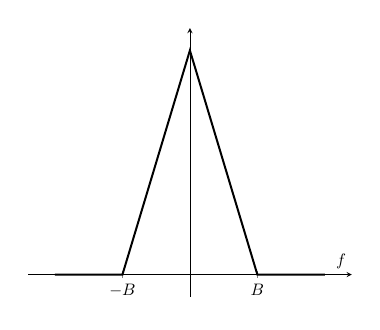
\begin{tikzpicture}[scale=.6]
		\begin{axis}[axis lines=middle,no markers,enlargelimits,xtick={-1,1},ytick={0},xticklabels={$-B$,$B$},xlabel={$f$}]
		\addplot [very thick]coordinates {(-2,0)(-1,0)(0,1)(1,0)(2,0)};
		\end{axis}\end{tikzpicture}}\qquad\subfloat[][$S_C(f)$] {
		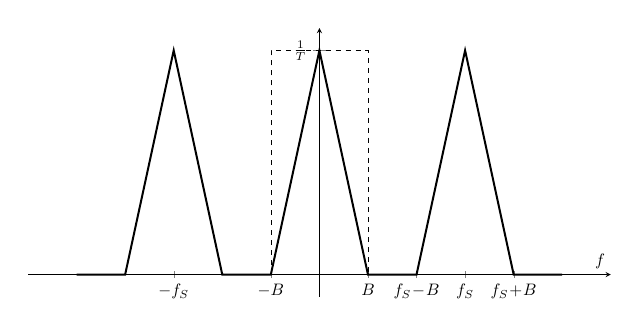
\begin{tikzpicture}[scale=.6]
		\begin{axis}[axis lines=middle,no markers,enlargelimits,xscale=1.8,xtick={-3,-1,1,2,3,4},ytick={1},xticklabels={$-f_S$,$-B$,$B$,$f_S\!-\!B$,$f_S$,$f_S\!+\!B$},yticklabels={$\frac{1}{T}$},xlabel={$f$}]
		\addplot [very thick]coordinates {(-5,0)(-4,0)(-3,1)(-2,0)(-1,0)(0,1)(1,0)(2,0)(3,1)(4,0)(5,0)};
		\addplot [dashed] coordinates{(-1,0)(-1,1)(1,1)(1,0)};
		\end{axis}\end{tikzpicture}
	}
	\caption{Esempio campionamento con $f_S\geq 2 B$}
\label{fig:campionamento}
\end{figure}

Per poter ricostruire il segnale è necessario che le repliche spettrali del segnale campionato non si sovrappongano al segnale in banda base, fenomeno detto \textsc{aliasing}. Deve essere $f_S-B\geq B$ ovvero la frequenza di campionamento deve essere almeno il doppio della banda unilatera del segnale
\begin{equation}
f_S\geq 2 B
\end{equation}
o, equivalentemente, definita \textsc{frequenza di Nyquist} $f_N=f_S / 2$, il segnale di partenza può essere ricostruito se la sua banda unilatera è $B<f_N$.

\begin{figure}[!h]
\centering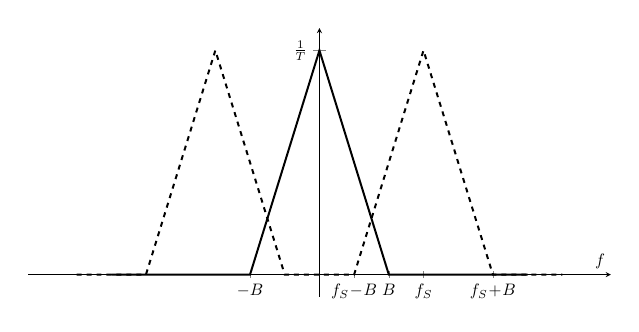
\begin{tikzpicture}[scale=.6]
\begin{axis}[axis lines=middle,no markers,enlargelimits,xscale=1.8,xtick={-1,.5,1,1.5,2.5},ytick={1},xticklabels={$-B$,$f_S\!-\!B$,$B$,$f_S$,$f_S\!+\!B$},yticklabels={$\frac{1}{T}$},xlabel={$f$}]
\addplot [very thick]coordinates {(-3,0)(-1,0)(0,1)(1,0)(3,0)};
\addplot [very thick,dashed]coordinates {(-3.5,0)(-2.5,0)(-1.5,1)(-.5,0)(.5,0)(1.5,1)(2.5,0)(3.5,0)};
\end{axis}\end{tikzpicture}
\caption{Esempio aliasing, campionamento con $f_S<2 B$}
\label{fig:aliasing}
\end{figure}
\end{proof}
\begin{esempio}
Un segnale audio con una banda $B=\SI{20}{\kilo\hertz}$ nella \textsc{Pulse Code Modulation (PCM)} viene campionato alle frequenze di $\SI{40}{\kilo\hertz}$ o $\SI{48}{\kilo\hertz}$.
\end{esempio}
\begin{nota}
Il segnale viene filtrato prima di essere campionato perché al segnale è sempre sovrapposto il rumore termico a tutte le frequenze.
\end{nota}
\begin{nota}
Se non è possibile campionare alla frequenza $f_S$ è necessario applicare un filtro di \emph{antialiasing} in una banda più stretta di $[-B,B]$, che fa perdere parte dell'informazione del segnale ma consente la ricostruzione seppur meno fedele del segnale originale.
\end{nota}

\subsection{Ricostruzione}

I campioni del segnale numerico giunti al ricevitore attraversano il \textsc{filtro di ricostruzione} per riottenere il segnale analogico di partenza. L'operazione di ricostruzione è necessaria per eliminare le repliche spettrali che non fanno parte dello spettro del segnale di partenza e che sono il risultato dell'operazione di campionamento.

Si utilizza un filtro passa basso ideale con banda pari alla frequenza di Nyquist, che faccia passare le frequenze comprese nell'intervallo $[-\frac{f_S}{2},\frac{f_S}{2}]$, e che compensi l'attenuazione di $\frac{1}{T}$ di $S_C(f)$, per l'eq.\ref{eq:filtro_passa_basso_ideale}
\begin{equation}
H(f)=T \rect{\frac{f}{f_S}}\qquad h(t)=\sinc{\frac{t}{T}}
\end{equation}

Il segnale ricostruito è la convoluzione del segnale campionato con il filtro
\begin{equation}\begin{split}
s_R(t)&=s_C(t)\ast h(t)=\intinf{s_C(\tau)h(t-\tau)}{\tau}=\\
&=\intinf{[s(\tau)\sum_{n=-\infty}^{+\infty}\impulse(\tau-n T)]\sinc{\frac{t-\tau}{T}}}{\tau}=\\
&=\intinf{\left[\sum_{n=-\infty}^{+\infty}s(n T)\impulse(\tau-n T)\right]\sinc{\frac{t-\tau}{T}}}{\tau}=\\
&=\intinf{\sum_{n=-\infty}^{+\infty}s(n T)\sinc{\frac{t-n T}{T}}\impulse(\tau-n T)}{\tau}=\\
\intertext{per la proprietà di setaccio dell'impulso l'integrale si riduce al valore in $\tau=n T$ si ha}
&=\sum_{n=-\infty}^{+\infty}s(n T)\sinc{\frac{t-n T}{T}}=\sum_{n=-\infty}^{+\infty}s(n T)\sinc{\frac{n T-t}{T}}
\end{split}
\end{equation}

Il segnale ricostruito nell'istante $t$ si ottiene come somma dei prodotti tra i campioni del segnale e il valore della funzione seno cardinale calcolata nei corrispondenti istanti di campionamento.

\begin{nota}
Se il segnale è passa banda, il teorema del campionamento continua a valere ma può essere impraticabile campionare al doppio della frequenza massima. In tal caso si sfruttano le repliche in banda base del segnale. Si seleziona una banda $B$ tale che la frequenza massima sia un multiplo intero della banda base, $\frac{f_M}{B}=m\in\N$, e si porrà $f_S\geq B$.
\end{nota}
\begin{nota}
Un campionamento perfetto dovrebbe estrarre l'informazione del segnale istantaneamente, mentre in realtà è necessario periodo di osservazione seppur breve. Un campionatore reale effettua la convoluzione del segnale con un rettangolo molto stretto, $s(t)\ast\rect{\frac{t}{\tau}}$ con un duty cycle molto piccolo, la cui trasformata risulta essere un $\Sinc$ molto ampio ($\frac{1}{\tau}\gg B$). Se in ricezione è richiesta alta fedeltà al segnale originale è sempre possibile equalizzare per compensare l'effetto sagomatore del filtro.
\end{nota}

\section{Campionamento di un processo aleatorio}
Sia il segnale analogico $x(t)$ membro di un processo aleatorio SSL. In queste condizioni è facile determinare il legame tra i momenti del primo e secondo ordine prima e dopo il campionamento del segnale. Infatti risulta
\[\E{X(t)} = \E{X(nT)} = \mu\]
Inoltre, per la funzione di autocorrelazione, si ha
\begin{align*}
R_X (\tau) &= \E{X(t)X(t-\tau)} \\
 R_{X_n} &= \E{X(nT)X\left((n-m)T\right)} = R_X(mT)
\end{align*}
Quindi per il campionamento di processi aleatori il valor medio della serie aleatoria $X(nT)$ coincide col valor medio del processo aleatorio tempo-continuo dal quale la serie è stata ottenuta per campionamento, mentre la funzione di autocorrelazione della serie aleatoria si ottiene mediante campionamento della funzione di autocorrelazione del processo aleatorio tempo-continuo.

\begin{figure}[!h]
	\centering
	\subfloat
	{
		\begin{tikzpicture}[>=latex']
		\node [block,node distance=1cm] (f) {campionamento};
		\node [left of= f,node distance=3cm](input) {$X(t)$};
		\node [right of= f,node distance=3cm] (output) {$X(nT)$};
		\node [below of= f,node distance=1.5cm] (t) {$T$};
		\draw [->] (input) -- (f);
		\draw [->] (f) -- (output);
		\draw [->] (t) -- (f);
		\end{tikzpicture}
	}
	\subfloat
	{
		\begin{tikzpicture}[>=latex']
		\node [block,node distance=1cm] (f) {campionamento};
		\node [left of= f,node distance=3cm](input) {$R_X(\tau)$};
		\node [right of= f,node distance=3cm] (output) {$R_X(mT)$};
		\node [below of= f,node distance=1.5cm] (t) {$T$};
		\draw [->] (input) -- (f);
		\draw [->] (f) -- (output);
		\draw [->] (t) -- (f);
		\end{tikzpicture}
	}
\caption{Campionamento di un processo aleatorio}
\label{fig:campionamento_processo_aleatorio}
\end{figure}

Inoltre, mediante trasformata di Fourier, il legame tra le funzioni di autocorrelazione si trasporta sulle rispettive densità spettrali di potenza (figure \ref{fig:campionamento} e \ref{fig:aliasing}):
\[
\fourier{R_X(\tau)} = \fourier{R_X(mT)} \implies S_{X}(f) =  S_{X_n}(f)
\]


\section{Quantizzazione}
L'operazione di \textsc{quantizzazione} trasforma i valori continui dei campioni del segnale appartenenti ad un intervallo $[-a,a]$ in valori discreti  dell'intervallo diviso in $Q$ livelli distinti di ampiezza $\Delta=\frac{2a}{Q}$.

Nei sistemi di elaborazione a logica binaria si assegna ad ogni campione del segnale un numero finito fisso di bit $N$ che consente di individuare $2^N$ livelli del segnale.

\begin{figure}[!h]
\centering
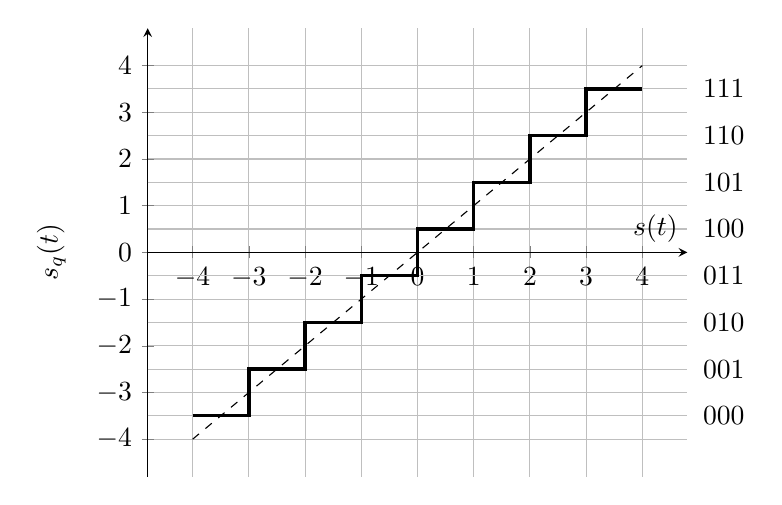
\begin{tikzpicture}
\begin{axis}[axis x line=middle,axis y line=left,enlargelimits,domain=-4:4,xlabel={$s(t)$},ylabel={$s_q(t)$},grid=major,xtick={-4,-3,-2,-1,0,1,2,3,4},ytick={-4,-3,-2,-1,0,1,2,3,4},extra y ticks={-3.5,-2.5,-1.5,-.5,0.5,1.5,2.5,3.5},extra y tick labels={$000$,$001$,$010$,$011$,$100$,$101$,$110$,$111$},extra y tick style={ticklabel pos=right}]
\addplot [const plot,very thick] coordinates {(-4,-3.5)(-3,-2.5)(-2,-1.5)(-1,-.5)(0,.5)(1,1.5)(2,2.5)(3,3.5)(4,3.5)};
\addplot [dashed] coordinates {(-4,-4)(4,4)};
\end{axis}
\end{tikzpicture}
\caption{Quantizzatore a 3 bit di segnale $s(t)\in[-4,4]$}
\end{figure}

L'operazione comporta una perdita di informazione irreversibile.

Dato un processo aleatorio stazionario il campionamento di una sua realizzazione $x(t)$ da luogo ad una variabile aleatoria, con la sua funzione densità di probabilità $f(x)$. Si supponga che la dinamica della v.a. assuma valori nell'intervallo $[-a,a]$, e che la quantizzazione in $Q$ livelli sia uniforme con intervalli di quantizzazione di ampiezza $\Delta=\frac{2a}{Q}$. I bordi degli intervalli si trovano in $x_i=-a+i\cdot\Delta$, con $i=0,\dots,Q$.  Per minimizzare l'errore di quantizzazione tra due intervalli successivi il livello assume valore intermedio
\begin{equation}
x_{i-1}\leq x<x_i,\,i=1,\dots,Q,\quad
x_q=\frac{x_i+x_i-1}{2}=-a+i\cdot\Delta-\frac{\Delta}{2}
\end{equation}
da cui risulta un errore di quantizzazione assoluto massimo di $\frac{\Delta}{2}$ in corrispondenza dei bordi degli intervalli.

L'operazione introduce quindi un rumore di quantizzazione che si può valutare con l'errore quadratico medio come
\[N_q=\E{(x-x_q)^2}=\intd{-a}{a}{(x-x_q)^2 f(x)}{x}=\sum_{i=1}^{Q}\intd{x_{i-1}}{x_i}{(x-x_q)^2 f(x)}{x}\]
Per un segnale con distribuzione uniforme si ha $f(x)=\frac{1}{2a},\,x\in[-a,a]$ e 0 altrove, da cui
\[\begin{split}N_q&=\sum_{i=1}^{Q}\intd{-a+(i-1)\Delta}{-a+i\Delta}{\left(x+a-i\Delta+\frac{\Delta}{2}\right)^2 \frac{1}{2a}}{x}=\\\intertext{ponendo $y=x+a-i\Delta+\frac{\Delta}{2}$}&=\frac{1}{2a}\sum_{i=1}^{Q}\intd{-\frac{\Delta}{2}}{\frac{\Delta}{2}}{y^2}{y}=\frac{Q}{2a}\bound{-\frac{\Delta}{2}}{\frac{\Delta}{2}}{\frac{y^3}{3}}=\frac{1}{\Delta}\frac{\Delta^3}{12}=\frac{\Delta^2}{12}
\end{split}\]
Tale quantità costituisce un disturbo che va confrontato con la potenza del segnale dato dallo spettro di potenza
\[S_x=\intd{-a}{a}{x^2\frac{1}{2a}}{x}=\frac{1}{2a}\bound{-a}{a}{\frac{x^3}{3}}=\frac{a^2}{3}=\frac{Q^2\Delta^2}{12}\]
Si ha il \textsc{rapporto segnale rumore di quantizzazione}
\begin{equation}
\frac{S_x}{N_q}=Q^2
\end{equation}
che migliora aumentando il numero di livelli di quantizzazione.
Per un numero di intervalli potenza di due si ha $\frac{S_x}{N_q}=2^{2n}$ che espresso in decibel \[\restrict{\frac{S_x}{N_q}}{\text{dB}}=10\Log 2^{2n}\cong n\cdot\SI{6}{\decibel}\]
ovvero si quadruplica il rapporto segnale rumore per ogni bit di quantizzazione in più.

Tale rapporto segnale rumore è stato calcolato per un processo con densità di probabilità uniforme, ma in generale la quantizzazione può essere non lineare, ad esempio per un processo gaussiano le cui realizzazioni si concentrano attorno al valor medio nullo e con varianza molto piccola. Per ottimizzare il rapporto segnale rumore di quantizzazione è necessaria una suddivisione più fine in livelli dove il segnale è più probabile, descrivendo i campioni con maggiore precisione.
